
\documentclass[11pt,oneside]{article} 

\usepackage{a4wide}

\usepackage{amsmath}
\usepackage{color}
%\usepackage{natbib} % kills arxiv 
\usepackage{framed}
%\usepackage{cite}
\usepackage{tikz}
\usepackage{tikz-cd}
%\usepackage{mathtools}

\RequirePackage{amsmath}
\RequirePackage{amssymb}
\RequirePackage{amsthm}
%\RequirePackage{algorithmic}
%\RequirePackage{algorithm}
%\RequirePackage{theorem}
%\RequirePackage{eucal}
\RequirePackage{color}
\RequirePackage{url}
\RequirePackage{mdwlist}

\RequirePackage{rotating}


\RequirePackage[all]{xy}
%\_CompileMatrices
%\RequirePackage{hyperref}
\RequirePackage{graphicx}
%\RequirePackage[dvips]{geometry}

\usepackage{xcolor}
\usepackage{amsmath,amsfonts,amssymb}
\usepackage{graphicx}
\usepackage[caption=false]{subfig}
\usepackage{enumerate}
\usepackage{mathrsfs}
\usepackage{mathtools}

% -------------- _Commands ----------------------

\makeatletter
\newcommand{\verbatimfont}[1]{\renewcommand{\verbatim@font}{\ttfamily#1}}
\makeatother

\newcommand{\Eref}[1]{(\ref{#1})}
\newcommand{\Fref}[1]{Fig.~\ref{#1}}
%\newcommand{\Aref}[1]{Appendix~\ref{#1}}
\newcommand{\SRef}[1]{Section~\ref{#1}}

\newcommand{\todo}[1]{\ \textcolor{red}{\{#1\}}\ }

\newcommand{\Aut}{\mathrm{Aut}}
\newcommand{\Stab}{\mathrm{Stab}}
\newcommand{\Fix}{\mathrm{Fix}}
\newcommand{\Orbit}{\mathrm{Orbit}}
\newcommand{\Ker}{\mathrm{Ker}}
\newcommand{\Image}{\mathrm{Im}}
\newcommand{\Dim}{\mathrm{Dim}}
\newcommand{\Tr}{\mathrm{Tr}}
\newcommand{\Det}{\mathrm{Det}}
\newcommand{\Complex}{\mathbb{C}}
\newcommand{\Integer}{\mathbb{Z}}
\newcommand{\GL}{\mathrm{GL}}
\newcommand{\Field}{\mathbb{F}}
\newcommand{\Code}{\mathcal{C}}
\newcommand{\End}{\mbox{End}}
\newcommand{\Inv}{\mbox{Inv}}
\newcommand{\Span}{\mbox{Span}}
\newcommand{\Hilb}{\mathcal{H}}
\newcommand{\Rey}{\mathcal{R}}
\newcommand{\tensor}{\otimes}

% Lemma, proof, theorem, etc.
\newcommand\nounderline[1]{ #1} 
\newcommand\dolemma[1]{\vskip 5pt \noindent{\bf \underline{Lemma #1.}\ }}
\newcommand\doproposition[1]{\vskip 5pt \noindent {\bf \underline{Proposition #1.}\ }}
\newcommand\dotheorem[1]{\vskip 5pt \noindent {\bf \underline{Theorem #1.}\ }}
\newcommand\docorollary[1]{\vskip 5pt \noindent {\bf \underline{Corollary #1.}\ }}
\newcommand\doexample[1]{\vskip 5pt \noindent {\bf \underline{Example #1.}\ }}
\newcommand\doproof{\vskip 5pt \noindent{\bf \nounderline{Proof:}\ }}

\newcommand\tombstone{\rule{.36em}{2ex}\vskip 5pt}

\newcounter{numitem}
\newcommand{\numitem}[1]{\refstepcounter{numitem}\thenumitem\label{#1}}

% braket notation...
\newcommand{\ket}[1]{|{#1}\rangle}
\newcommand{\expect}[1]{\langle{#1}\rangle}
\newcommand{\bra}[1]{\langle{#1}|}
\newcommand{\ketbra}[2]{\ket{#1}\!\bra{#2}}
\newcommand{\braket}[2]{\langle{#1}|{#2}\rangle}

% Categories
\newcommand{\Set}{\mathbf{Set}}
\newcommand{\FinSet}{\mathbf{FinSet}}
\newcommand{\GSet}{\mathbf{GSet}}
\newcommand{\GRep}{\mathbf{GRep}}

\newcommand{\thinplus}{\!+\!}
\newcommand{\MM}{\mathcal{M}}

\renewcommand{\arraystretch}{1.2}



\title{Algebraic Morse theory for quantum codes}

\author{Simon Burton}

\date{\today}

\flushbottom

\begin{document}

\maketitle

\section{Introduction}

As application of these techniques, we suggest/conjecture the following connections:
\begin{enumerate}
\item[(i)]
Alternate description of logical operators in
generalized surface codes \cite{Delfosse2016}.
\item[(ii)]
Use to derive the unitary encoding circuits in \cite{Higgott2020}.
\item[(iii)]
Explain the appearence of ZX-calculus in \cite{deBeaudrap2020}.
\item[(iv)]
Gaussian elimination and finite geometries \cite{Rengaswamy2018}.
\end{enumerate}


\section{Algebraic Morse theory}

We review algebraic Morse theory 
\cite{Jollenbeck2005,Kozlov2005,Skoldberg2006}.
Consider a chain complex $C$ over a field $K$:
$$
    C_N \xrightarrow{\partial_N} C_{N-1}
    \to ...
    \to C_1 \xrightarrow{\partial_1} C_0.
$$
Pick a basis $X_i$ for each $C_i$
and let $X=\sqcup X_i$.
Define a weighted directed graph $\Gamma_C$
with vertex set $X$ and
weighted edge $u\xrightarrow{w}v$
for every $u\in X_i, v\in X_{i-1}$
where $w = (\partial_i)_{v,u} \ne 0.$

A {\it matching} $\MM$ is any collection of
edges from $\Gamma_C$ such that 
any two distinct edges in $\MM$ do not share a vertex.
Let $\Gamma_C^\MM$ be the graph obtained from
$\Gamma_C$ by replacing every edge $u\xrightarrow{w} v\in \MM$
with $v\xrightarrow{-1/w} u.$
A matching $\MM$ is {\it Morse} when
$\Gamma_C^\MM$ contains no (directed) cycles.

Fix a Morse matching $\MM.$
Let $X_i^\MM$ be the set of elements of $X_i$ not found in
any edge of $\MM.$
These elements are called {\it critical.}
Let the vector space $C_i^\MM$ be generated from the basis $X_i^\MM.$
We define a new chain complex, the {\it Morse complex},
as follows:
%\begin{align*}
%\partial_i^\MM : C_i^\MM &\to C_{i-1}^\MM \\
%    c \in X_i^\MM &\mapsto \sum_{c'\in X_{i-1}^\MM} \Gamma(c, c') c'.
%\end{align*}
$$
\begin{array}{lll}
\partial_i^\MM : &C_i^\MM &\to\ \  C_{i-1}^\MM \\
    & c \in X_i^\MM &\mapsto \displaystyle\sum_{c'\in X_{i-1}^\MM} \Gamma(c, c') c'.
\end{array}
$$
Here $\Gamma(c,c')$ is the sum over the weights of all 
paths in $\Gamma_C^\MM$ from $c$ to $c'$.
Any path in $\Gamma_C^\MM$ 
$$
c_1 \xrightarrow{w_1} c_2 \xrightarrow{w_2} ...  \xrightarrow{w_r} c_r
$$
has weight
$$
w(c_1 \xrightarrow{w_1} c_2 \xrightarrow{w_2} ...  \xrightarrow{w_r} c_r)
= \prod_{i=1}^r w_i.
$$

\dolemma{\numitem{Lem}} 
%The maps $\{ \partial_i^\MM \}_{i=0}^N$ define a chain complex.
The maps $\partial_\star^\MM$ define a chain complex.
\doproof 
See \cite{Jollenbeck2005} Lemma 2.1.
\tombstone

%Define chain maps $f:C_\star\to C_\star^\MM$ and $g:C_\star^\MM\to C_\star$ as
Now define the following linear maps:
$$
\begin{array}{lll}
f_i : &C_i &\to\ \  C_i^\MM \\
    & c \in X_i &\mapsto \displaystyle\sum_{c'\in X_i^\MM} \Gamma(c, c') c',\\
g_i : &C_i^\MM &\to\ \  C_i \\
    & c \in X_i^\MM &\mapsto \displaystyle\sum_{c'\in X_i} \Gamma(c, c') c'. \\
\chi_i : &C_i &\to\ \  C_{i+1} \\
    & c \in X_i &\mapsto \displaystyle\sum_{c'\in X_{i+1}} \Gamma(c, c') c'.
\end{array}
$$

\dolemma{\numitem{Lem}}
$f_\star:C_\star\to C_\star^\MM$ and $g_\star:C_\star^\MM\to C_\star$ 
are chain maps, ie.
\begin{align*}
    \partial^\MM f &= f \partial \\
    \partial g &= g \partial^\MM.
\end{align*}
\doproof See \cite{Jollenbeck2005} Lemma 2.2.
\tombstone

\dolemma{\numitem{Lem}}
The maps $f_\star$ and $g_\star$ define a homotopy
equivalence between $C$ and $C^\MM$ with
chain homotopies $\chi:g f\to I_C$ and $0:f g\to I_{C^\MM}$.
This means we have
\begin{align*}
    g_i  f_i - I_C &= \partial_{i+1} \chi_i + \chi_{i-1}\partial_i,\\
    f_i  g_i - I_{C^\MM} &= 0.
\end{align*}
\doproof See \cite{Jollenbeck2005} Lemma 2.3.
\tombstone

\dotheorem{\numitem{Lem}}
The homologies for $C$ and $C^\MM$ are isomorphic:
$$
    H_\star(C) \cong H_\star(C^\MM).
$$
\doproof
Immediate consequence of the above lemmas.
\tombstone


\section{Examples}

In the following examples we set $K={\mathbb F}_2$.

{\bf Example 1.}
A planar graph, with six vertices, 
$X_0=\{v_1,v_2,v_3,v_4,v_5,v_6 \}$
and seven edges, 
$X_1=\{e_1,e_2,e_3,e_4,e_5,e_6,e_7\}$.
A Morse matching $\MM$ is shown with thick orange arrows.
The critical cells are $X_{\star}^\MM = \{ v_6, e_1, e_4 \}.$
These are marked with a red circle.

\begin{center}
\begin{tabular}{cc}
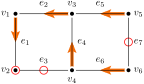
\includegraphics[]{images/pic-complex-graph} &
\ \ \ \ \ 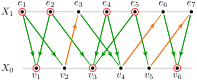
\includegraphics[]{images/pic-poset-graph} \\
A planar graph & 
\ \ \ \ \ $\Gamma_C^\MM$
\end{tabular}
\end{center}

\begin{center}
\includegraphics[]{images/pic-matrix-graph}
\end{center}

The Morse matchings on a graph $G$ are in one-to-one
correspondence with the set of rooted forests of $G$,
see~\cite{Chari2005} Prop.~3.1.


% From Chari2005:
%    In particular, the facets of the complex M(Γ) correspond
%    precisely to the rooted spanning trees of Γ. Each facet
%    gives rise to a “different” proof of the elementary facet
%    that a (connected) graph with m edges and n nodes is
%    homotopy equivalent to a wedge of m-n+1 circles. The
%    rooted spanning tree (in isolation) can be collapsed
%    according to the orientation to a point represented by
%    the root node. The rest of the m-n+1 edges form the m-n+1
%    critical 1-cells giving the homotopy type. 

\noindent
{\bf Example 2.}
This is a tetrahedron, with vertices $X_0=\{v_1,v_2,v_3,v_4\}$,
edges 
$X_1=\{e_1,e_2,e_3,e_4,e_5,e_6\}$,
and faces 
$X_2=\{f_1,f_2,f_3,f_4\}.$
The critical cells are $X_{\star}^\MM = \{ v_1, f_4 \}.$
The face $f_4$ is shown on the left as streched out to infinity.

\begin{center}
\begin{tabular}{cc}
\includegraphics[]{images/pic-complex-tetra} & 
\ \ \ \ \ \includegraphics[]{images/pic-poset-tetra} \\
A tetrahedron &
\ \ \ \ \ $\Gamma_C^\MM$ 
\end{tabular}
\end{center}


\noindent
{\bf Example 3.}


\begin{center}
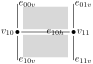
\includegraphics[scale=0.8]{images/pic-complex-surface}
\end{center}



\bibliography{refs}{}
\bibliographystyle{abbrv}



\end{document}



